% MyLaTeXDocument.tex
\documentclass[12pt]{article}

% Preamble.tex
\usepackage[english]{babel}									
\usepackage[utf8]{inputenc}								
\usepackage[T1]{fontenc}
\usepackage{comment}
\usepackage{amsmath,amsfonts,amssymb,amsthm,cancel,siunitx,
calculator,calc,mathtools,empheq,latexsym}
\usepackage{subfig,epsfig,tikz,float}		          
\usepackage{booktabs,multicol,multirow,tabularx,array}
\usepackage{listings}
\usepackage{hyperref,url}
\hypersetup{
    colorlinks=true,
    linkcolor=blue,
    citecolor=blue,
    filecolor=magenta,      
    urlcolor=cyan,
}
\setlength{\parindent}{0pt}
\setlength{\parskip}{5pt}
\textwidth 13.5cm
\textheight 19.5cm
\columnsep .5cm

\newcommand{\shellcmd}[1]{\\\indent\indent\texttt{\footnotesize\# #1}\\}
         % Put packages and new definitions etc in Preamble.tex

\title{Getting started with Git (and \LaTeX)}
\author{Graham W. Wilson}

\begin{document}

\date{}
\maketitle

% Abstract.tex
\vspace{-0.5cm}
% Abstract
\bigskip
\noindent
{Almost minimal working example (MWE) of using git. 
Also included are some examples of using {\LaTeX}  
for equations, figures, tables, and references. 
You can see this project on Overleaf with 
this Overleaf shared link 
\href{https://www.overleaf.com/read/xjwwvcsyywdq}{https://www.overleaf.com/read/xjwwvcsyywdq}.
}

\baselineskip=\normalbaselineskip
         % Short summary of the document  (Abstract.tex)

% Body.tex
\section{Git/GitHub}\label{sec:1}

Git is a distributed version control system similar 
in functionality to earlier incarnations like cvs and svn. It is 
the de facto standard in software development 
and for scientific computing. It is used for tracking software 
changes and for coordinating concurrent work 
on associated projects amongst multiple people. 
For most of our class use case, we will deal with the 
simple workflow of personal use rather than collaborative use.

For each project, we will use GitHub as 
the remote software repository, and a 
local Git client like the git command line interface (CLI) 
on Ubuntu to manage Git transactions.

A pre-requisite is a GitHub account. 
This includes a username, password 
and secondary authentication mechanism.
For the latter, I use https based authentication using 
a Personal Access Token (PAT); this is a 40 character 
automatically generated secondary password. 
Make sure you do not publish your PAT!

Once you have the above setup, you can create 
a new remote project repository by going to your github web page 
(github.com/yourusername), being logged in (with your password and possibly PAT), go 
to ``Repositories'' link on the top, and 
click on the green ``New'' button. This will create 
the new repository with the project name 
you assigned - for example ``ProjectileMotion''. When 
you go to that repository, there should be another green 
button marked ``Code''. This gives a number of methods for cloning your 
remote repository locally on your computer.
My preference is to use https, namely,

\texttt{git clone https://github.com/yourusername/ProjectileMotion.git}

This will copy the entire remote repository named ProjectileMotion to 
a folder/directory with that name to your current local path. 
So if you are at \texttt{/home/yourusername}, the git directory 
will be at \texttt{/home/yourusername/ProjectileMotion}.

You can then navigate to that folder by doing, 

\texttt{cd ProjectileMotion}

and use the code or add more code content.

It is always a good idea to check the status of your local repository, especially 
after making changes.

\texttt{git status}

Especially before, but also after executing git commands.

If you have new or modified files that you want to 
be included in your next update (commit) of the repository you 
need to ``add'' these changes, either one file at a time,

\texttt{git add specific-file.txt}

or usually all at once (all files at current path and below).

It is OK (and often very desirable) to not 
have all files under git control. This can be managed 
using a \texttt{.gitignore} hidden file.

Often you will want to add all 
files all at once (all files at current path and below), one can do this using

\texttt{git add .}

Another \texttt{git status} here would help confirm what got added 
and this is a good time to undo any mistakes. (The files that 
were in red should now be in green.

Now we are ready to commit the changes to your local repository, 
including a short "commit" comment. 

\texttt{git commit -m "My commit message"}

One can also break the changes into smaller thematic chunks.

In order to ``publish'' or synchronize your local repository changes to the 
remote repository (GitHub) one needs to ``push'' the changes to GitHub. This needs 
authentication with your GitHub username and PAT (for https). 
It is possible to cache your GitHub credentials locally for 
up to 10 hours (so that the username/PAT do not need 
to be respecified in further local-to-remote transactions).

\texttt{git push}

There is of course more functionality (and complications) 
to Git/GitHub than described above, and various more 
advanced workflows, but these are some of the essential steps 
for single person use. For me, some of the main reasons to use this 
are as a backup, and as a straightforward way to use 
the same code on different machines.

\section{Getting more out of Git}
Five additional useful commands are:

\begin{enumerate}
    \item \texttt{git pull - -dry-run}
    (the two dashes preceding dry should have no space in the middle...).
    This shows what would happen if 
    you were to update your local repository with any changes made to the remote repository, like for 
    example feedback files I may have added, and serves as a check on whether there 
    are any new changes. 
    If there are no new changes there will be no output from the command. 
    \item \texttt{git pull} This does update your local repository with any changes made to 
    the remote repository. For example if you downloaded the ClassExamples repository last week 
    and want the latest, do git pull from the ClassExamples local directory.
    \item \texttt{git diff filename.txt} See what changes there are between your locally modified  version of the file and the one in the (reference) remote repository.
    \item \texttt{git log} History of all the commits and commit messages made to this repository.
    \item \texttt{git config - -global credential.helper 'cache - -timeout=36000'}. This will cache your authentication credentials for up to 10 hours after initial authentication, meaning you only need to enter your username and password once in a session. (above two-dash remark applies twice here).
    This works for me on my laptop and the room 2076 Ubuntu system but could be OS and git 
    client dependent.
\end{enumerate}

\section{\LaTeX}
\LaTeX is a document preparation system that can handle documents ranging 
from basic notes, to lab reports, to technical documents, 
scientific papers and textbooks. It is especially strong 
in focusing the author on the content and the structure 
of the document, rather on details of typesetting and 
what ends up on specific pages. It is the tool of choice 
for documents with equations.

It used to have a reasonably steep learning curve, because it needs to be compiled 
rather being WYSIWYG (what-you-see-is-what-you-get). Now there are LaTeX 
integrated development environments (IDEs) like Overleaf that allow one 
to add content and visualize the type-set document essentially instantaneously.
Overleaf has become particularly powerful for working in a team on a common document.
To get started with Overleaf you will need an account.

\section{Some {\LaTeX} examples}

The Rayleigh distribution has the following probability density function,
\begin{equation}\label{eq:11}
p(r;\sigma) = \frac{r}{\sigma^2} \exp(-r^{2}/(2\sigma^2)
\end{equation}
where $r \ge 0$ and $\sigma$ is known as the scale parameter. 
It relates to the magnitude of a bi-variate 
uncorrelated Gaussian distribution. An example of random numbers drawn from 
this distribution is shown in Fig.~\ref{fig:ray}.

\begin{figure}[!htb]
\centering
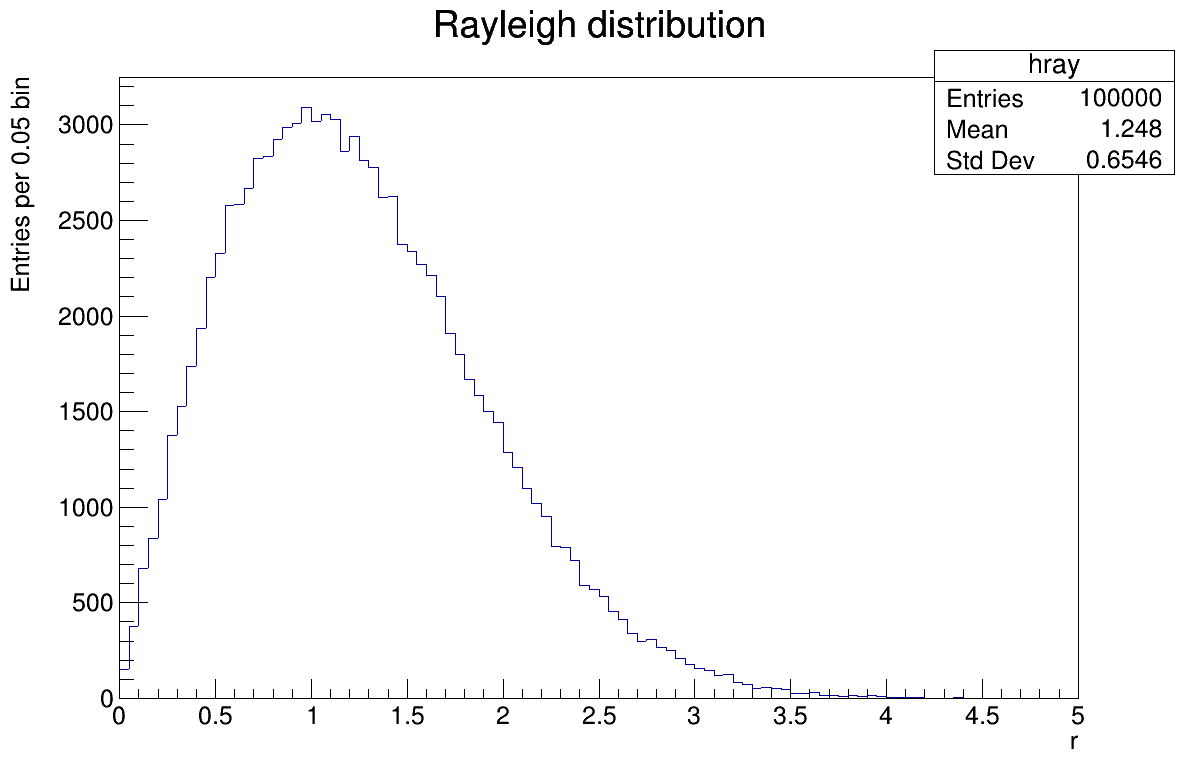
\includegraphics[width=0.8\textwidth]{hray.png}
\caption{Random numbers following the Rayleigh distribution with scale parameter, $\sigma=1$.}
\label{fig:ray}
\end{figure}

An environment tabularx, an extension of tabular, creates 
a paragraph-like column whose width automatically expands so that 
the declared width of the environment is filled. 
Table \ref{table:tab1} shows a minimal working example.

\newcolumntype{C}{>{\centering\arraybackslash}X}
\begin{table}[!htb]
\centering
\caption{Example table.}
\begin{tabularx}{1.0\textwidth}{ C | C | C | C }
\toprule
Case & Method\#1 & Method\#2 & Method\#3 \\ 
\midrule
1 & 50 & 837 & 970 \\
2 & 47 & 877 & 230 \\
3 & 31 & 25 & 415 \\
4 & 35 & 144 & 2356 \\
5 & 45 & 300 & 556 \\
\bottomrule
\end{tabularx}
\label{table:tab1} 
\end{table}

\section{Previous work}\label{sec:2}

There are many ways to reference bibliographic information. Here I used a style file 
from the CMS experiment. The references below are taken verbatim 
from an Overleaf template.

A simple \LaTeX{} example of one author was written by \cite{moretti2003weighted}
and several authors by \cite{bechara1986use}.
A book can be cited by \cite{kleinrock1975queueing}.
A much longer \LaTeX{} example was written by \cite{maculan2003integer}.
An example of a technical report was written by \cite{HoracioYanasse}.
             % You could subdivide Body.tex further if you want. For 
                         % example one file per section. 
                         % This divide and conquer strategy may also be good 
                         % for finding and fixing compilation errors

% References.tex. These use BibTeX and a style file from the CMS experiment
\bibliographystyle{CMS-lucas}
\bibliography{references.bib}
       % References.tex has the commands that define the 
                         % way the references are defined and cited

\end{document}
